% !TEX encoding = UTF-8 Unicode
\documentclass[a4paper]{article}
\usepackage[utf8]{inputenc}
\usepackage[T1]{fontenc}
\usepackage[francais]{babel}
\usepackage{fullpage}
\usepackage{hyperref}
\usepackage{verbatim}
\usepackage{graphicx}
\usepackage[nonumberlist]{glossaries}
\usepackage{amssymb,amsmath}
\usepackage{subfig}
\usepackage{float}
\title{{\textsc{INFO-F-302} : Informatique Fondamentale} \\ Projet - Rapport}
\author{Jérôme \textsc{Hellinckx} \\ Thomas \textsc{Herman}}

\begin{document}
\renewcommand{\labelitemi}{$\bullet$}

\maketitle

\section{Le problème}
Le problème de base consiste à essayer d'enchâsser un ensemble de rectangles dans la surface d'un grand rectangle. Ce problème se complexifie au fil des questions posées. 

\section{Définitions}
Quelques termes et notations utilisés dans ce rapport : 
\begin{itemize}
	\item \textit{largeur}, la dimension verticale d'un rectangle ;
	\item \textit{longueur}, la dimension horizontale d'un rectangle ;
	\item $R$ le grand rectangle dans lequel les autres rectangles doivent être enchâssés ;
	\item $ n,m \in \mathbb{N}_{>0} $ la largeur et longueur du rectangle $R$ ;
    \item l'ensemble $N = \{0,\dots,n\} \mapsto \mathbb{N}$, l'ensemble des naturels $\leq n$ ;
    \item l'ensemble $M = \{0,\dots,m\} \mapsto \mathbb{N}$, l'ensemble des naturels $\leq m$ ;
        \item l'ensemble $H = \{0,\dots,h\} \mapsto \mathbb{N}$, l'ensemble des naturels $\leq h$ ;
	\item l'ensemble $K = \{r_1,\dots ,r_k\}$ de $k$ rectangles $r$ plus petits que $R$ ;
	\item $\mathcal{X}:\{1,\dots,k\} \mapsto \mathbb{N}_{>0} $, fonction nous donnant la longueur d'un rectangle ;
	\item $\mathcal{Y}:\{1,\dots,k\} \mapsto \mathbb{N}_{>0} $, fonction nous donnant la largeur d'un rectangle ;
	\item $\mu :\{1,\dots,k\} \mapsto \{1,\dots,m\}\times\{1,\dots,n\}$ fonction d'assignation d'un rectangle à une position contenue dans $R$ tel que si $\mu(i) \mapsto (a,b)$ alors les sommets du rectangle $r_i$ sont $(a,b), (a,\mathcal{Y}(i)+b), (\mathcal{X}(i)+a,\mathcal{Y}(i)+b), (\mathcal{X}(i)+a,b)$.\\
	
	
\end{itemize}


Variables booléennes utilisées :
\begin{itemize}
	\item $\sigma_{k,a,b}$, vrai ssi le rectange $k$ est placé en $(a,b)$ (coin inférieur gauche du rectangle)
	
\end{itemize}
\section{Questions}
\subsection{Écrire les contraintes en langage mathématique}
\begin{enumerate}
	\item $\forall i \in \{1,\dots, k\}, \mu(i) \mapsto (a,b), a\in M, b\in N : a+\mathcal{X}(i) \leq m $
	\item $\forall i \in \{1,\dots, k\}, \mu(i) \mapsto (a,b), a\in M, b\in N : b+\mathcal{Y}(i) \leq n $
	\item $\forall i, j \in \{1,\dots, k\},  i \neq j, \mu(i) \mapsto (a, b),  \mu(j) \mapsto (d,e) :  a + \mathcal{X}(i) \leq d \lor a \geq d +\mathcal{X}(j) \lor b + \mathcal{Y}(i) \leq e \lor b \geq e + \mathcal{Y}(j) $
\end{enumerate}

\newpage
\subsection{Construire une formule $\Phi$ en FNC de la logique propositionnelle}
Notons que les notations $(a, b)$ et $(d, e)$ utilisées sont les mêmes que celles exprimées en langage mathématique.
Rappelons que $\sigma_{k,a,b}$ valué à 1 signifie que le rectangle $k$ est placé en $(a,b)$. Dès lors, traduire la première contrainte en FNC revient à interdire une valuation de 1 pour $\sigma_{k,a,b}$ si le triplet $(k, a, b)$ est hors bornes :
\begin{equation*}
\begin{split}
	&C_1 = \bigwedge\limits_{\substack{k\in K}} \bigwedge\limits_{\substack{a \in M, \\ a > m - \mathcal{X}(k) \\ b\in N}} \lnot \sigma_{k,a, b}\\
    &C_2 = \bigwedge\limits_{\substack{k\in K}} \bigwedge\limits_{\substack{a \in M \\ b \in N,\\ b > n - \mathcal{Y}(k)}} \lnot \sigma_{k,a, b}
\end{split}
\end{equation*}

Vient ensuite la contrainte de superposition. En logique propositionnelle cette contrainte s'écrit sous la forme $\sigma_{k,a,b} \rightarrow \lnot \sigma_{l,d,e}$ si $(a,b)$ et $(d,e)$ se superposent pour $k$ et $l$ donnés. Déterminer si ces couples se superposent revient à vérifier si $a-\mathcal{X}(l) < d < a +\mathcal{X}(k)$ et $b-\mathcal{Y}(l) < e < b +\mathcal{Y}(k)$. En FNC nous obtenons alors :
\begin{equation*}
C_3 = 	\bigwedge\limits_{\substack{k\in K}}
			\bigwedge\limits_{\substack{a \in M \\ b \in N}}
				\bigwedge\limits_{\substack{l\in K,\\ l > k}}
					\bigg[
					\bigwedge\limits_{\substack{d \in M,\\ a-\mathcal{X}(l) < d < a +\mathcal{X}(k) \\  e \in N, \\b-\mathcal{Y}(l) < e < b +\mathcal{Y}(k)}}
						\lnot \sigma_{k,a,b} \lor \lnot \sigma_{l,d,e}	
					\bigg]
\end{equation*}

Ajoutons également une contrainte "au moins une", aisée à construire en FNC : 
\begin{equation*}
	C_4 = \bigwedge\limits_{k\in K} \bigvee\limits_{\substack{a\in M \\ b \in N}} \sigma_{k,a,b}
\end{equation*}

La mise en FNC complète de $\Phi$ est donc :
\begin{equation*}
 \bigwedge\limits_{i \in \{1, 2, 3, 4\}} C_i
\end{equation*}

\subsection{Implémentation et tests}
Pour résoudre le problème de base (i.e. la question 2) avec \textsc{Minisat}, nous utilisons la variable \texttt{mu[k][a][b]} qui est analogue à $\sigma_{k,a,b}$. Nous appliquons alors les contraintes décrites pour $\sigma_{k,a,b}$ ci-dessus à cette variable. Pour récupérer la solution du \texttt{solver} (si elle existe), nous parcourons alors cette variable \texttt{mu[k][a][b]} et dès que nous trouvons $V(\texttt{mu[k][a][b]}) = 1$ nous mettons $\mu(k) \mapsto (a,b)$ et nous passons au $k$ suivant. L'implémentation peut se trouver dans le fichier \texttt{OrthogonalPackingSolver.cpp}.
\subsubsection{Utilisation de l'implémentation}
Notre implémentation est utilisable de deux manières :
\begin{enumerate}
	\item en lançant directement l'exécutable \texttt{./solver} après un appel à \texttt{make}. Dans ce cas un menu s'affichera pour configurer le programme en fonction de la question. Une fois le choix effectué, il faudra entrer manuellement la description du problème (format définit plus bas) ;
	\item en utilisant le script \texttt{run.sh} fournit. Il s'agira ici de d'abord changer les permissions du fichier (\texttt{chmod +x run.sh}) avant de l'exécuter. De plus, il est possible de fournir des arguments au script pour configurer la question d'une part et donner un fichier contenant un problème d'autre part. Par exemple, pour résoudre le problème décrit dans le fichier \texttt{data/example1.opp} avec la configuration de la question 3 (problème de base, 2D sans contrainte supplémentaire) il suffit d'entrer 
\begin{center}
\texttt{./run.sh 3 data/example1.opp}
\end{center}
\end{enumerate}

\paragraph{Format d'entrée du problème}
L'entrée attendue (manuelle ou dans un fichier en utilisant \texttt{run.sh}) est la même que dans l'énoncé. Exemple pour instancier un problème où $k=2$, $n=4$, $m=4$, $\mathcal{X}(1) = 4$, $\mathcal{Y}(1) = 1$, $\mathcal{X}(2) = 1$, $\mathcal{Y}(2) = 4$ (voir aussi \texttt{data/example1.opp}):
\texttt{\\2\\4\\4\\1 4 1\\2 1 4}

\paragraph{Format de sortie de la solution}
À nouveau, le format de sortie respecté est celui décrit dans l'énoncé. Si aucune solution n'est trouvée, le programme affiche \texttt{0}, sinon le programme affiche les fonctions $\mu(k) \mapsto (a,b)$ pour tout k. Exemple de sortie avec le fichier \texttt{data/example2.opp} :
\texttt{\\1 0 2\\2 2 0 \\3 0 0}

\subsubsection{Visualisation de la solution}
Parallèlement à l'affichage via \texttt{stdout}, le programme lancera également (si une solution existe) une visualisation de la solution en s'aidant d'un \textit{binding} \texttt{python} que nous avons écrit. Le script \texttt{python} appelé utilise \texttt{matplotlib} qui est installable via \texttt{pip install matplotlib} sous \texttt{OS X} ou \texttt{sudo apt-get install python-matplotlib} sous \texttt{Linux}. Le code \texttt{python} se trouve dans le fichier \texttt{plot\_opp.py}. 
Ainsi, en exécutant les commandes \texttt{./run.sh 3 data/example2.opp} et \texttt{./run.sh 3 data/q3\_8x8.opp} le programme affichera : 

\begin{figure}[H]
  \centering
  \subfloat[\texttt{data/example2.opp}]{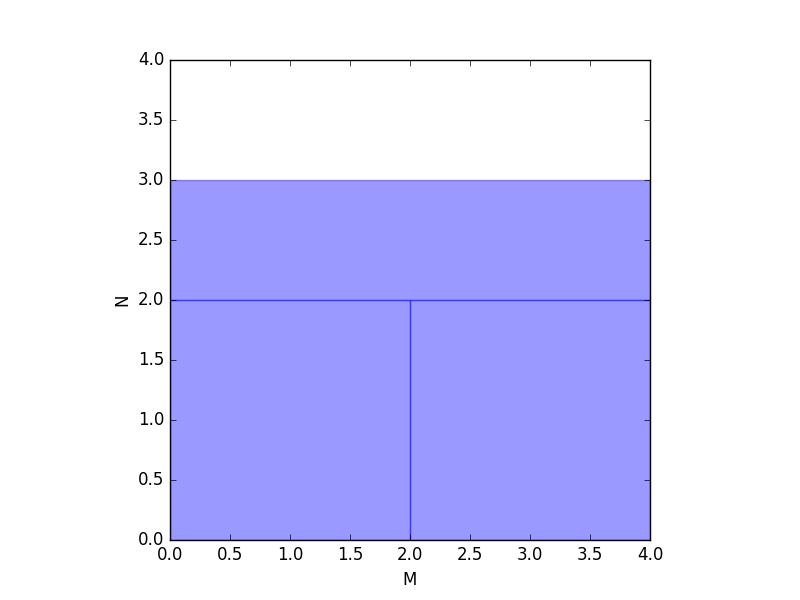
\includegraphics[width=0.4\textwidth]{example2.png}\label{fig:f1}}
  \hfill
  \subfloat[\texttt{data/q3\_8x8.opp}]{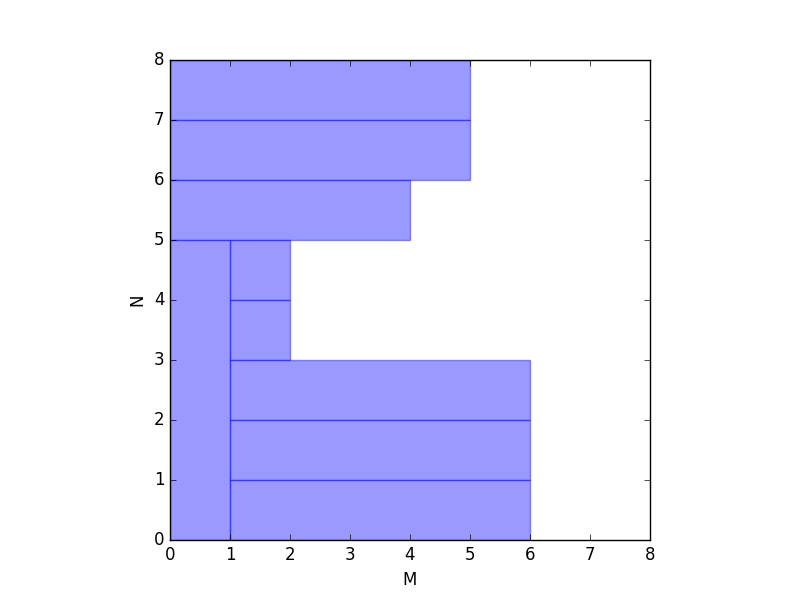
\includegraphics[width=0.4\textwidth]{q3_8x8.png}\label{fig:f2}}
  \caption{Exemples d'affichage}
\end{figure}

\subsection{Calculer la longueur minimum du carré $R$ admettant une solution}
Tout d'abord, il faut pouvoir déterminer un $n$ de départ pour lequel il est certain qu'une solution soit satisfaisable. Pour ce faire, nous introduisons $n_{max}$. Cette nouvelle variable représente le maximum entre la somme de toutes les longueurs de chaque rectangle de $K$ d'une part, et d'autre part la somme de leurs largeurs. Elle est donc calculée de la manière suivante:
\begin{equation*}
n_{max} = max ( \sum_{i=0}^k \mathcal{X}(i) , \sum_{i=0}^k \mathcal{Y}(i) )
\end{equation*}
Ensuite, nous introduisons également $n_{min}$, le $n$ minimal théorique. Cette variable correspond à la racine carrée de la somme des aires de chaque rectangle de $K$. En effet, cela correspond au scénario idéal dans lequel il n'y a aucun espace entre les rectangles (mais n'est pas toujours réalisable suivant la dimension des rectangles). Elle est calculée de la manière suivante:
\begin{equation*}
n_{min} = \sqrt[]{ \sum_{i=0}^k \mathcal{X}(i) * \mathcal{Y}(i) }
\end{equation*}
Nous appellerons ici $n$ dimension. Nous avons donc une dimension maximale pour laquelle il est certain d'avoir une solution et une dimension minimale théorique. 
Introduisons donc deux nouvelles variables:
\begin{itemize}
\item $\eta_{n}$ qui est vrai ssi $n$ est une dimension \textit{acceptable} avec $n_{min} <= n <= n_{max}, n \in \mathbb{N}_{>0}$ ;
\item $\rho_{k,a,b,n}$ qui est vrai ssi le rectangle $r_k$ placé en $(a,b)$ ne dépasse pas le carré $R$ de dimension $n$  avec $k \in K, a \in M, b \in N, n_{min} <= n <= n_{max}, n \in \mathbb{N}_{>0}$.\\
\end{itemize}

Au niveau de l'implémentation, le programme génère $n_{min}$ et $n_{max}$, $n$ et $m$ ne sont donc pas donnés. Au départ, toutes les dimensions sont considérées acceptables et le programme utilise une variable $n_{courant}$ pour déterminer la plus grande dimension acceptable. Le programme boucle alors en appelant \texttt{solver.solve()} tant que $\Phi$ est satisfaisable, signifiant qu'une solution ayant comme carré $R$ avec dimension $n_{courant}$ existe. La variable $n_{courant}$ est alors décrémentée. Dès que $\Phi$ n'est plus satisfaisable, $n_{courant} + 1$ renseigne sur la dimension de $R$ minimale.
Il faut donc rajouter deux contraintes. La première stipulant que $\sigma_{k,a,b}$ est vrai ssi on a au moins un $n$ pour laquelle $\rho_{k,a,b,n}$ est vrai :
\begin{equation*}
C_5 = \bigwedge\limits_{i\in K} \bigwedge\limits_{\substack{a \in M \\ b \in N}} \sigma_{k,a,b} \lor \bigg[ \bigvee\limits_{n_{min} <= n <= n_{max}} \rho_{k,a,b,n} \bigg]
\end{equation*}
Et la deuxième, utilisant $\eta_n$, stipulant que si $\rho(k,a,b,n)$ est vrai, alors $\eta(n)$ doit être vrai :
\begin{equation*}
C_6 = 	\bigwedge\limits_{\substack{k\in K}}
			\bigwedge\limits_{n = n_{min}}^{n_{max}}
				\bigwedge\limits_{\substack{a \in M, \\ 0 <= a < n - \mathcal{X}(k) \\ b \in N, \\ 0 <= b < n - \mathcal{Y}(k)}}
					\big[
						\lnot \rho_{k,a,b,n} \lor \eta_n
					\big]
\end{equation*}
Précisons par souci de clarté que chaque itération rajoute une clause $\lnot \eta_{n_{courant}}$ pour donc mettre la dimension $n_{courant}$ comme non-acceptable. 
Notons enfin qu'il faut aussi ajouter une contrainte mettant $\rho(k,a,b,n)$ à faux si $(a,b)$ est hors des bornes avec $R$ de dimension $n$. Ceci est cependant tout à fait similaire aux contraintes $C_1$ et $C_2$ en ajoutant à gauche $\bigwedge\limits_{n_{min} <= n <= n_{max}}$.

\subsection{Calculer la longueur minimum du carré $R$ avec $r_i$ de taille $i\times i \ \forall i \leq n$}
Nous pouvons considérer qu'il s'agit d'un cas particulier de la question précédente. En effet, la seule différence est qu'avant de calculer le $n_{min}$ et le $n_{max}$, il faut générer les rectangles (qui cette fois-ci sont des carrés) en fonction du nombre $k$ de rectangles lus en $input$. Ensuite, la résolution est similaire à la question 4 ci-dessus.


\subsection{Ajout d'une troisième dimension}
Par soucis de compréhension, notons tout d'abord le développement de la fonction d'assignation $\mu :\{1,\dots,k\} \mapsto \{1,\dots,m\}\times\{1,\dots,n\}\times\{1,\dots,h\}$ et donc nous utiliserons $\mu(i) \mapsto (a, b, c)$ et $ \mu(j) \mapsto (d, e, f)$.
Nous appliquons ensuite le même raisonnement que celui utilisé pour déterminer les contraintes en deux dimensions. Nous considérons dans un premier temps la contrainte triviale qui sert à border la hauteur des rectangles $\{r_1,\dots ,r_k\}$ entre $0$ et la hauteur $h$ de $R$ :
\begin{equation*}
    C_7 = \bigwedge\limits_{\substack{k\in K}} \bigwedge\limits_{\substack{a \in M \\ b \in N\\ c\in H, \\ c > h - \mathcal{Z}(k)}} \lnot \sigma_{k,a, b, c}
\end{equation*}
Mettons maintenant à jour les contraintes $C_1$, $C_2$ et $C_4$ afin qu'elles prennent en compte la troisième dimension:
\begin{equation*}
\begin{split}
	&C'_1 = \bigwedge\limits_{\substack{k\in K}} \bigwedge\limits_{\substack{a \in M, \\ a > m - \mathcal{X}(k) \\ b\in N \\ c\in H}} \lnot \sigma_{k,a, b, c}\\
    &C'_2 = \bigwedge\limits_{\substack{k\in K}} \bigwedge\limits_{\substack{a \in M \\ b \in N,\\ b > n - \mathcal{Y}(k) \\ c\in H}} \lnot \sigma_{k,a, b, c}\\
    &C'_4 = \bigwedge\limits_{k\in K} \bigvee\limits_{\substack{a\in M \\ b \in N \\ c \in H}} \sigma_{k,a,b,c}
\end{split}
\end{equation*}
Pour finir, nous adaptons $C_3$ définie lors de la construction de $\Phi$ précédente en remarquant que si un rectangle $r_1$ se trouve \textit{plus haut} ou \textit{plus bas} qu'un rectangle $r_2$, $r_1$ et $r_2$ ne se superposent pas. Répétons que cette observation est directement déduite de $C_3$ qui devient alors :
\begin{equation*}
	C'_3 = 	\bigwedge\limits_{\substack{k\in K}}
			\bigwedge\limits_{\substack{a \in M \\ b \in N \\ c \in H}}
				\bigwedge\limits_{\substack{l\in K,\\ l > k}}
					\bigg[
					\bigwedge\limits_{\substack{d \in M,\\ a-\mathcal{X}(l) < d < a +\mathcal{X}(k) \\  e \in N, \\b-\mathcal{Y}(l) < e < b +\mathcal{Y}(k)\\ f \in H, \\ c-\mathcal{Z}(l) < f < c+\mathcal{Z}(k)}}
						\lnot \sigma_{k,a,b,c} \lor \lnot \sigma_{l,d,e,f}	
					\bigg]
\end{equation*}


\subsection{Ajout de contraintes qui ne fassent pas flotter les parallélépipèdes}
Pour qu'un parallélépipède $k$ ne flotte pas, si $\mu(k) \mapsto (a,b,c)$ il faut que sa composante $c$ vale soit $0$, soit qu'il existe un $l$ avec $\mu(l) \mapsto (d,e,f)$ tel que $f = c - \mathcal{Z}(l)$ et les couples $(a,b), (d,e)$ se superposent :
\begin{equation*}
C_8  = 	\bigwedge\limits_{\substack{k\in K}}
			\bigwedge\limits_{\substack{a \in M \\ b \in N \\ c \in H_{>0}}}
			\bigg[
				\lnot \sigma_{k,a,b,c} \lor
				\bigvee\limits_{\substack{l\in K, \\ l \neq k}}
				\Big[
					\bigvee\limits_{\substack{d \in M,\\ a-\mathcal{X}(l) < d < a +\mathcal{X}(k) \\  e \in N, \\b-\mathcal{Y}(l) < e < b +\mathcal{Y}(k)}}
						\sigma_{l,d,e,c - \mathcal{Z}(l)}	
				\Big]
			\bigg]
\end{equation*}


\subsection{Solution avec pivot}
\subsection{Minimum de $p$ unités de contact entre les rectangles et les bords de $R$}
Il est nécessaire de d'abord déterminer si un rectangle $r_i$ touche un des bords du rectangle $R$, c'est-à-dire si un de ses côtés touche un bord de $R$. Nous obtenons donc que $r_i$ touche $R$ si  $\forall i \in \{1,\dots, k\}, \mu(i) \mapsto (a,b) :  (a = 0) (\lor a+ \mathcal{X}(i) = m) \lor (b = 0) \lor (b + \mathcal{Y}(i) = n)$. Il faut ensuite faire le somme de chaque côté de $r_i$ qui touche un bord de $R$ (si nous posons qu'une unité $p$ vaut $1$). Pour traduire cette contrainte en FNC, nous définissons la variable $\omega_{i,p}$ qui est vrai ssi les rectangles $\{r_1,\dots ,r_i\} \subseteq K$ au minimum $p$ unités de contact avec les bords de R : 
\begin{equation*}
C_9 =  \bigwedge\limits_{i\in K} 
\end{equation*}

\end{document}